\documentclass[../main.tex]{subfiles}
\begin{document}
\chapter{Introduction To Groups}
\section{Examples and Definitions}
You can think about groups in two ways:
\begin{itemize}
  \item Algebra
  \item Symmetries
\end{itemize}
\subsection{A Symmetries Viewpoint}
Consider the symmetries of an equilateral triangle:
\begin{itemize}
  \item The ``do-nothing'' symmetry (identity)
  \item Rotational symmetry of order 3. (Rotate $120^\circ$ clockwise or anti-clockwise)
  \item Reflective symmetry across three different axes
\end{itemize}
This gives a total of 6 symmetries.
Informally a symmetry is an action that does not change the overall shape.
\begin{remark}
  A regular $n$-gon has $2n$ symmetries.
\end{remark}
We can compose multiple symmetries to get composite symmetries.
If we label the vertices of the triangle we can identify which of the original symmetries the composite symmetry is equivalent to.

To invert a reflection you can just repeat the same reflection, they are ``self-inverse''.
\begin{remark}[Important Features]
  \begin{itemize}
    \item Symmetries can be \textbf{composed} to get another symmetry (\textbf{closed})
    \item There is an \textbf{identity} ``do-nothing'' symmetry
    \item Every symmetry has an \textbf{inverse}
    \item Composition of symmetries is \textbf{associative} ($a \circ (b \circ c) = (a \circ b) \circ c$)
  \end{itemize}
\end{remark}
\begin{remark}[Warning]
  Composition of symmetries is \textbf{not} always \textbf{commutative}.
  
  For example, if we rotate and then reflect it is not the same as if we reflect and then rotate.
\end{remark}
\subsection{An Algebraic Viewpoint}
\begin{definition}[Binary Operation]
  A \textit{binary operation} on a set $X$ is a function $\cdot: X \times X \to X$.
  This means for $x, y \in X$, $(x, y) \mapsto x \cdot y$
\end{definition}
\begin{definition}[Group]
  A \textit{group} is a triple $(G, \cdot, e)$ where:
  \begin{itemize}
    \item $G$ is a set
    \item $\cdot$ is a binary operation on $G$
    \item $e \in G$
  \end{itemize}
  such that the following 4 group axioms are satisfied:
  \begin{enumerate}
    \item \textbf{Closure -} For all $a, b \in G$, $a \cdot b \in G$
    \item \textbf{Associativity -} For all $a, b, c \in G$, $(a \cdot b) \cdot c = a \cdot (b \cdot c)$
    \item \textbf{(Right) Identity -} There exists an $e \in G$ such that for all $a \in G$, $a \cdot e = a$
    \item \textbf{(Right) Inverses -} For all $a \in G$ there exists $b \in G$ such that $a \cdot b = e$
  \end{enumerate}
\end{definition}
We noticed earlier that the symmetries of the equilateral triangle form a group.
We can also think about this definition as encompassing algebra with a single operation.
\begin{example}
  $(\Z, +, 0)$ forms a group.
  \begin{enumerate}
    \item \textbf{Closure -} For all $a, b \in \Z$, $a + b \in \Z$ \tick
    \item \textbf{Associativity -} We know that addition is associative \tick
    \item \textbf{Identity -} 0 is the identity as for all $a \in \Z$, $a + 0 = a$ \tick
    \item \textbf{Inverses -} The inverse of an element $a \in \Z$ is $-a$ (which is also in $\Z$) as $a + (-a) = 0$ \tick
  \end{enumerate}
\end{example}
The definition of a group has some important consequences:
\begin{proposition}
  Let $(G, \cdot, e)$ be a group and let $a, b, b', e' \in G$.
  \begin{enumerate}
    \item if $a \cdot b = e$ then $b \cdot a = e$. (Right inverses are left inverses)
    \item $e \cdot a = a$ (The right identity is also left identity)
    \item If $a, b, b'$ are such that $a \cdot b = e = a \cdot b'$ then $b = b'$ (Inverses are unique)
    \item If $a \cdot e' = a$ then $e' = e$ (The identity is unique)
  \end{enumerate}
  \label{groupProp}
\end{proposition}
\begin{proof}[\textbf{i}]
 \begin{align*}
   b &= b \cdot e \text{ by identity axiom} \\
     &= b \cdot (a \cdot b) \text{ by assumption} \\
     &= (b \cdot a) \cdot b \text{ by associativity}
 \end{align*}
 By the inverse axiom, $\exists c \in G$ such that $b \cdot c = e$.
 We can now right multiply by $c$.
 \begin{align*}
  b \cdot c &= ((b \cdot a) \cdot b) \cdot c \\
            &= (b \cdot a) \cdot (b \cdot c) \text{ by associativity} \\
          e &= (b \cdot a) \cdot e \text{ by definition of $c$} \\
            &= b \cdot a \text{ by identity axiom}
 \end{align*}
 So $b \cdot a = e$ as rquired.
\end{proof}
\begin{proof}[\textbf{ii}]
  By inverses and \textbf{i} there is a $b \in G$ such that $a \cdot b = e = b \cdot a$ so:
  \begin{align*}
    e \cdot a &= (a \cdot b) \cdot a \\
              &= a \cdot (b \cdot a) \text{ by associativity} \\
              &= a \cdot e \text{ as above} \\
              &= a \text{ by identity axiom} \\
  \end{align*}
  So $e \cdot a = a$ as required and therefore the identity is both a right and left identity.
\end{proof}
\begin{proof}[\textbf{iii}]
  \begin{align*}
    b' &= e \cdot b' \text{ by \textbf{ii}} \\
       &= (b \cdot a) \cdot b' \text{ by \textbf{i}} \\
       &= b \cdot (a \cdot b') \text{ by associativity} \\
       &= b \cdot e \text{ by assumption} \\
       &= b \text{ by identity axiom}
  \end{align*} 
  So $b  = b'$ as required and therefore inverses are unique.
\end{proof}
\begin{proof}[\textbf{iv}]
  By the inverse axiom and \textbf{i}, $\exists b \in G$ such that $b \cdot a = e$.
  Working from $a \cdot e' = a$:
  \begin{align*}
    a &= a \cdot e'\\
    b \cdot a &= b \cdot (a \cdot e') \\
              &= (b \cdot a) \cdot e' \text{ by associativity} \\
              &= e \cdot e' \text{ as above} \\
              &= e' \text{ by part \textbf{ii}}
  \end{align*}
  Since $b \cdot a = e$ also, it follows that $e = e'$ as required and so the identity is unique.
\end{proof}
\begin{remark}[Notation]
  Part \textbf{iii} of \cref{groupProp} states that inverses are unique.
  Therefore if $a \cdot b = e$ we may write $b = a^{-1}$.
\end{remark}
So from part \textbf{i} we have that:
\[
  a \cdot a^{-1} = e = a^{-1} \cdot a
\]
which means that:
\[
  (a^{-1})^{-1} = a
\]
It makes sense to extend this further to more familiar notation:
\begin{remark}[Notation]
  For any $a \in G$ define:
  \begin{itemize}
    \item $a^{0} = e$
    \item $a^{n} = a^{n - 1} \cdot a$ for any $n \in \N$
    \item $a^{-n} = (a^{-1})^{n}$ for any $n \in \N$
  \end{itemize}
\end{remark}
\begin{proposition}
  For $a \in G$, $m, b \in \Z$:
  \begin{enumerate}
    \item $a^{m} \cdot a^{n} = a^{m + n}$
    \item $(a^{m})^{n} = a^{mn}$
  \end{enumerate}
\end{proposition}
\begin{proof}[\textbf{i}]
  \begin{align*}
    a^{m} \cdot a^{n} &= (a^{m - 1} \cdot a) \cdot (a^{n - 1} \cdot a) \\
                      &= ((a^{m - 2} \cdot a) \cdot a) \cdot ((a^{n - 2} \cdot a) \cdot a) \\
                      &\;\; \vdots \quad\text{repeating and dropping brackets because of associativity} \\
                      &= \underbrace{(a \cdot a \cdot \cdots \cdot a)}_{\text{$a$ applied $m$ times}} \cdot \underbrace{(a \cdot a \cdot \cdots \cdot a)}_{\text{$a$ applied $n$ times}} \\
                      &= \underbrace{a \cdot a \cdot \cdots \cdot a}_{\text{$a$ applied $m + n$ times}} \\
                      &\; \; \vdots \quad\text{regrouping and reintroducing brackets} \\
                      &= (a^{m + n - 2} \cdot a) \cdot a \\
                      &= a^{m + n - 1} \cdot a \\
                      &= a^{m + n}
  \end{align*} 
\end{proof}
\begin{proof}[\textbf{ii}]
  \begin{align*}
    (a^{m})^{n} &= (a^{m - 1} \cdot a)^{n} \\
                &\; \; \vdots \quad\text{repeating and dropping brackets because of associativity}\\
                &= {\underbrace{(a \cdot a \cdot \cdots \cdot a)}_{\text{$a$ applied $m$ times}}}^{n} \\
                &= {\underbrace{(a \cdot a \cdot \cdots \cdot a)}_{\text{$a$ applied $m$ times}}}^{n - 1} \cdot \underbrace{(a \cdot a \cdot \cdots \cdot a)}_{\text{$a$ applied $m$ times}} \\
                &\; \; \vdots \quad\text{repeating and dropping brackets because of associativity}\\
                &= \underbrace{a \cdot a \cdot \cdots \cdot a}_{\text{$a$ applied $mn$ times}} \\
                &\; \; \vdots \quad\text{regrouping and reintroducing brackets} \\
                &= a^{mn}
  \end{align*}
\end{proof}
\begin{remark}[Warning]
Recall that it is \textbf{not necessarily} true that $a \cdot b = b \cdot a$.
Because of this it is \textbf{not necessarily} true that $(a \cdot b)^{-1} = a^{-1} \cdot b^{-1}$.
\end{remark}
However we can still find the inverse of $a \cdot b$.
Consider:
\begin{align*}
  (a \cdot b) \cdot (b^{-1} \cdot a^{-1}) &= \left((a \cdot b) \cdot b^{-1}\right) \cdot a^{-1} \\
                                          &= \left(a \cdot (b \cdot b^{-1})\right) \cdot a^{-1} \\
                                          &= (a \cdot e) \cdot a^{-1} \\
                                          &= a \cdot a^{-1} \\
                                          &= e
\end{align*}
So $(a \cdot b)^{-1} = b^{-1} \cdot a^{-1}$.
\begin{definition}[Abelian Group]
  If $(G, \cdot, e)$ is a group and its binary operation is commutative, i.e.
  \[
    a \cdot b = b \cdot a \quad \forall a, b \in G
  \]
  then $G$ is and \textit{abelian group}.
\end{definition}
\begin{example}[Trivial Group]
  If $G = \{ e \}$ and $e \cdot e = e$, then $(G, \cdot, e)$ is called the \textit{trivial group}.
\end{example}

\subsection{Familiar Examples}
To help us categorise groups we must first define the order of a group:
\begin{definition}[Group Order]
  The \textit{order} of a group $(G, \cdot, e)$  is the number of elements of $G$.
  We denote this $|G|$ or $\#G$.
\end{definition}
\begin{definition}[Finite/Infinite Group]
  If $|G| < \infty$ then $(G, \cdot, e)$ is a \textit{finite group}.
  Otherwise $(G, \cdot, e)$ is an \textit{infinite group}.
\end{definition}
Here are some examples/non-examples of groups:
\subsubsection{Infinite Groups}
\begin{enumerate}
  \item $(\Z,  +, 0)$, $(\Q, +, 0)$, $(\R, +, 0)$, $(\C, +, 0)$ are all abelian groups.
    In each case, the inverse of $x$ is $-x$.
  \item $(\N, +, 0)$ is \textbf{not} a group as inverses do not exist for elements other than $0$.
  \item $(\Q, \times, 1)$ is \textbf{not} a group as $0$ has no inverse.
    However if we just remove 0, $(\Q \setminus \{0\}, \times, 1)$ is a abelian group!

    Similarly, $(\R \setminus \{0\}, \times, 1)$ and $(\C \setminus \{0\}, \times, 1)$ are abelian groups.
\end{enumerate}
\subsubsection{Finite Groups}
\begin{enumerate}
  \item For any $n \in \N$ let $C_n = \{z \in \C : z^{n} = 1\}$ then $(C_n, \times, 1)$ is an abelian group.
  \item Let $\Z_n = \{0, 1, 2, \ldots, n - 1\}$ and let $a +_n b$ be the remainder when $a + b$ is divided by $n$ (i.e. the value of $a + b$ under mod $n$).
    Then $(\Z_n, +_n, 0)$ is an abelian group.

    Closure holds as the remainder $r$ when dividing by $n$ is in the range $0 \leq r \leq n - 1$.
    The inverse of a general element $a$ is given by $n - a$ so that $a + (n - a) \equiv 0 \pmod{n}$.
\end{enumerate}
\section{Symmetric Groups}
\begin{definition}[Bijection]
  Let $X, Y$ be sets, a \textit{bijection} is a map $f: X \to Y$ that has an inverse $g: Y \to X$ such that $f \circ g = 1=\id_Y$ (i.e. $(f \circ g)(y) = y$ for all $y \in Y$) and $g \circ f = \id_X$ (i.e. $(f \circ g)(y) = y$ for all $y \in Y$).
\end{definition}
\begin{remark}[Notation]
  $(f \circ g)(y) = f(g(y))$ by definition.
\end{remark}
\begin{definition}[Permutation]
  A \textit{permutation} is a bijection $X \to X$ (i.e. from $X$ to itself).
\end{definition}
\begin{definition}[Symmetry Group]
  $\Sym(X)$ is defined to to be the set of permutations of a set $X$.
\end{definition}
\begin{lemma}
  Composition of functions is associative.

  That is, for maps of sets:
  \[
    W \xrightarrow{f} X \xrightarrow{g} Y \xrightarrow{h} Z
  \]
  Then $(h \circ g) \circ g = h \circ (g \circ f)$
  \label{assocLemma}
\end{lemma}
\begin{proof}
For any $w \in W$,
  \[
    ((h \circ g) \circ f)(w) = (h \circ g)(f(w)) = h(g(f(w))) = h((g \circ f)(w)) = (h \circ (g \circ f))(w)
  \]
  as required.
\end{proof}
This makes it easy to see that $\Sym(X)$ is a group.
\begin{proposition}
  For any set $X$, $(\Sym(X), \circ, \id_X)$ is a group.
\end{proposition}
\begin{proof}
  \begin{enumerate}
    \item \textbf{Closure -} Automatic, note that $(f \circ g)^{-1} = g^{-1} \circ f^{-1}$.
    \item \textbf{Associativity -} Follows from \cref{assocLemma}.
    \item \textbf{Identity -} $\id_X: X \to X$, $x \mapsto x$ is an identity.
    \item \textbf{Inverses -} Inverses exist by definition of bijectivity.
  \end{enumerate}
\end{proof}
\begin{definition}
  If $X = \{1, 2, \ldots, n\}$ then we write $S_n = \Sym(X)$.
\end{definition}
\begin{example}
  \begin{enumerate}
    \item $S_3$ is the group of ways permuting three objects.
    \item $S_{52}$ is the group of ways of shuffling a deck of cards.
  \end{enumerate}
\end{example}
\begin{remark}
  $|S_n| = n!$
\end{remark}
\begin{remark}[Notation]
  Writing  $(G, \cdot, e)$ for a group is cumbersome.
  Henceforth we will usually just write $G$.

  If we want to emphasise that $e$ is the identity element of $G$, we will write $e_G$.
  Similarly we can also write $\cdot_G$ for the operation on $G$.
\end{remark}

\section{Subgroups}
Sometimes, we want to restrict our attention to smaller groups. For example, $\Z$ inside $\R$ or just the rotations of a triangle instead of all symmetries.
\begin{definition}[Subgroup]
  Let $G$ be a group and $H \subseteq G$. If the following hold:
  \begin{enumerate}
    \item $e \in H$
    \item $a \cdot b \in H$ for all $a, b \in H$
    \item $a^{-1} \in H$ for all $a \in H$
  \end{enumerate}
  Then we say that $H$ is a \textit{subgroup} of $G$ and we write $H \leq G$.
\end{definition}
\begin{remark}
  If $G$ is a group and $H \leq G$ then $H$ is a group.
\end{remark}
\begin{example}
  There are two easy examples of subgroups:
  \begin{enumerate}
    \item Every group $G$ is a subgroup of itself
    \item For any group $G$, $1_G = \{e_G\}$ is the trivial subgroup of $G$.
  \end{enumerate}
\end{example}
\begin{definition}[Proper Subgroup]
  $H$ is a \textit{proper subgroup} of $G$ if $H \leq G$, but $H$ is not $G$ itself or the trivial subgroup.
  We denote this $H < G$.
\end{definition}
\subsection{Subgroups of the Integers}
\begin{example}
  For $n \in \N_0$ define:
  \[
    n\Z = \{nk : k \in \Z\} = \{\ldots, -2n, n, 0, n, 2n, \ldots\}
  \]
  Now:
  \begin{enumerate}
    \item \textbf{Identity -} $0 \in n\Z$.
    \item \textbf{Closure -} Let $x = nk$, $y = nl \in n\Z$ then $x + y = n(k + l) \in n\Z$
    \item \textbf{Inverses -} Let $x = nk \in n\Z$ then $-x = -nk = n(-k) \in n\Z$
  \end{enumerate}
  Therefore $n\Z \leq \Z$.
  In fact, these are \textbf{all} of the subgroups of $\Z$.
\end{example}
\begin{proposition}
  If $H$ is a subgroup of $\Z$ then $H = n\Z$ for some $n \in \N_0$.
\end{proposition}
\begin{proof}
  \begin{proofcases}
    \begin{case}{$H = \{0\}$}
      If $H = \{0\}$ then $H = 0\Z$ and we are done.
    \end{case}
    \begin{case}{Otherwise}
      We may choose $n \in H \setminus \{0\}$ to be the smallest positive $n \in H$.

      (Note that if $x \in H$ and $x < 0$ then $-x \in H$ and $-x > 0$. So unless $H = \{0\}$, H must contain a positive number)

      By induction, we see that $nk \in H$ for all $k \in \Z^{+}$.
      By inverses, $-n$ is also in $H$, so by induction again we see that $-nk \in H$ for all $k \in \Z^{+}$.
      So $n\Z \subseteq H$.

      We can now proceed by contradiction.
      Suppose $n\Z \neq H$, so there is some $x \in H$ such that $x \notin n\Z$.
      That is, $x$ is not a multiple of $n$.
      Using the division algorithm, we get that $x = nq + r$ for some $q \in \Z$ and $0 < r < n$.
      But now $r = x - nq$ and both $x \in H$ and $nq \in n\Z \subseteq H$ so $r \in H$.
      But $0 < r < n$ so this contradicts the assumption that $n$ was the smallest non-zero element of $H$.
      Thus $H = n\Z$.
    \end{case}
  \end{proofcases}
\end{proof}
\subsection{Other Examples of Subgroups}
\begin{example}
  \begin{enumerate}
    \item If $H, K \leq G$ then $H \cap K \leq G$. (See Example Sheet 1, Q2)
    \item For any family of subgroups $H_i \leq G$, $\bigcap_{i}^{} H_i$ is a subgroup of $G$.
  \end{enumerate}
\end{example}
\section{Generating Sets}
\begin{definition}[Subgroup Generated by $X$]
  Let $X$ be a subset of a group $G$. Then:
  \[
    \langle X \rangle = \bigcap_{X \subseteq H \leq G}^{} H
  \]
  Is the intersection of all subgroups of $G$ that contain $X$.
  It is called the \textit{subgroup generated by $X$}.
\end{definition}
If $G = \langle X \rangle$ we say that $X$ generates $G$, or $X$ is a generating set for $G$.
Intuitively $\langle X \rangle$ is the smallest subgroup of $G$ containing $X$.
If $X$ generates $G$, it means that every $g \in G$ can be written as:
\[
  g = x^{\pm 1}_{1} x^{\pm 1}_{2} \cdots x^{\pm 1}_{n}
\]
For some $n \geq 0$ where are $x_i \in X$ and are not necessarily unique.
Note that when $n=0$ the empty product is interpreted as the identity element. (See Example Sheet 1, Q9)
\section{Isometries}
Let $\C$ be the plane, equipped with with the usual notion of Euclidean distance:
\[
   |z-w| = \sqrt{(z_1 - w_1)^2 + (z_2 - w_2)^2}, \quad z = z_1 + i z_2, w = w_1 + i w_2
\]
\begin{definition}[Isometry]
  For any subset $X \subseteq \C$, an \textit{isometry} of $X$ is a bijection $f: X \to X$ that preserves distance:
  \[
    |f(x) - f(y)| = |x - y| \quad \forall x, y \in X
  \]
\end{definition}
\begin{proposition}[Isometry Groups in $\C$]
  Let $X \subseteq \C$.
  The set of isometries of $X$, $\Isom(X)$, is a subgroup of $\Sym(X)$.
  In particular $\Isom(X)$ is a group.
\end{proposition}
\begin{proof}
  We need to check $\Isom(X)$ against  the definition of a subgroup.
  Let $f, g \in \Isom(X)$ and $x, y \in X$.
  \begin{enumerate}
    \item \textbf{Identity -} $\id_X \in \Isom(X)$ as doing nothing clearly preserves distance.
    \item \textbf{Closure -} Since $f, g$ are isometries, we need to consider what $f \circ g$ does to distance:
      \[
        |f(g(x)) - f(g(y))| = |g(x) - g(y)| = |x - y|
      \]
      So $f \circ g \in \Isom(X)$.
    \item \textbf{Inverses -} We know that $f^{-1}$ exists as we defined $f$ to be a bijection.
      Let $x' = f^{-1}(x), y' = f^{-1}(y)$, because $f$ is an isometry:
      \[
        |x' - y'| = |f(x') - f(y')|
      \]
      So:
      \[
        |f^{-1}(x) - f^{-1}(y)| = |f(f^{-1}(x)) - f(f^{-1}(y))| = |x - y|
      \]
      and therefore $f^{-1} \in \Isom(X)$.
  \end{enumerate}
\end{proof}
\section{Dihedral Groups}
\subsection{Definition}
\begin{definition}[Dihedral Groups]
  Let $X_n \subseteq \C$ be the $n$-gon with vertices at:
  \[
    \{e^{\frac{2k\pi i}{n}}: k = 0, 1, \ldots, n-1\} \text{ for } n \geq3
  \]
  Then $D_{2n}$ is defined to be $\Isom(X_n)$.
\end{definition}
\begin{example}
  $D_6$ is the symmetry group of an equilateral triangle that we studied earlier.
\end{example}
We would like to show that $|D_{2n}| = 2n$.
The proof of this will also give us a good description of all the elements of $D_{2n}$.

\subsection{Geometric Lemmas}
To do this, we first need some geometric lemmas.
The first of which is a basic fact from Euclidean geometry.
\begin{lemma}[Kite Lemma]
  Let $x_1, x_2, y_1, y_2 \in \C$. If:
  \[
    |y_1 - x_1| = |y_2 - x_1| \text{ and } |y_1 - x_2| = |y_2 - x_2|
    \label{kiteLemma}
  \]
  then $x_2 - x_1$ is orthogonal to $y_2 - y_1$.
\end{lemma}
\begin{center}
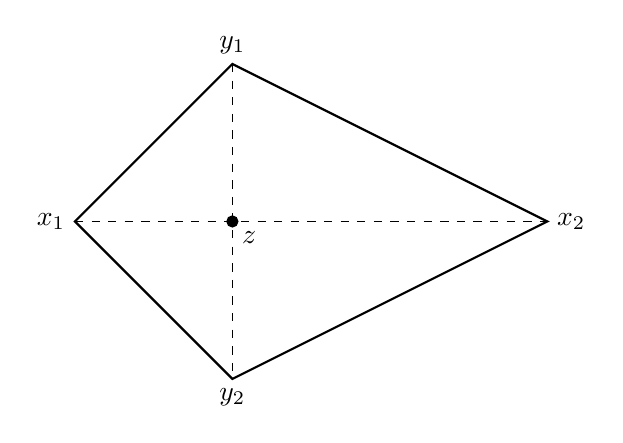
\begin{tikzpicture}[scale=2]
  \coordinate (z) at (-0.5,0);
  \coordinate (x1) at (-1.5,0);
  \coordinate (x2) at (1.5,0);
  \coordinate (y1) at (-0.5,1);
  \coordinate (y2) at (-0.5,-1);

  \draw[thick] (y1) -- (x1) -- (y2) -- (x2) -- cycle;

  \draw[dashed] (y1) -- (y2);
  \draw[dashed] (x1) -- (x2);

  \filldraw[black] (z) circle (1pt);

  \node[above] at (y1) {\(y_1\)};
  \node[below] at (y2) {\(y_2\)};
  \node[left] at (x1) {\(x_1\)};
  \node[right] at (x2) {\(x_2\)};
  \node[below right] at (z) {\(z\)};
\end{tikzpicture}
\end{center}
\begin{proof}
  By symmetry $\angle x_1 z y_1$ = $\angle x_1 z y_2$ but $y_1 y_2$ is a straight line so the two angles must sum to $\pi$ and thus they must be $\pi/2$ individually.
\end{proof}
\begin{lemma}[Three Point Lemma]
  Let $X \subseteq \C$ and $f \in \Isom(X)$ if there are $x_1, x_2, x_3 \in X$ that are \textbf{not collinear}, such that $f(x_i) = x_i$ for $i = 1, 2, 3$, then $f = \id_X$
  \label{threePoint}
\end{lemma}
\begin{proof}
  Proceed by contradiction.
  Suppose $f(y) \neq y$ for some $y \in X$.
  Then:
  \begin{align*}
    |f(y) - x_i| &= |f(y) - f(x_i)| \text{ by hypothesis} \\
                 &= |y - x_i| \text{ since $f$ is an isometry}
  \end{align*}
  for $i =1, 2, 3$.

  Now by \cref{kiteLemma} (Kite Lemma), with $y_1 = y$ and $y_2 = f(y)$. $x_2 - x_1$ is perpendicular to $y_2 - y_1 = f(y) - y$.
  But similarly using \cref{kiteLemma} again, $x_3 - x_1$ is perpendicular to $f(y) - y$.
  So both $x_2 - x_1$ and $x_3 - x_1$ are perpendicular to the same thing.
  Hence $x_1, x_2, x_3$ are collinear which contradicts the hypothesis.
\end{proof}
\begin{remark}
  There is equally an $n + 1$ point lemma which is valid in $\R^{n}$.
\end{remark}
\subsection{Elements of \texorpdfstring{$D_{2n}$}{Dihedral Groups}}
To prove the theorem we need to define two elements of $D_{2n}$:
\begin{enumerate}
 \item Rotation by $2\pi/n$, $r(z) = e^{\frac{2\pi i}{n}}z$.
 \item Reflection in the real axis, $s(z) = z^{*}$.
\end{enumerate}
We can now tackle the theorem which classifies the elements of $D_{2n}$:
\begin{theorem}
  For $n \geq 3$, $|D_{2n}| = 2n$ and:
  \[
    D_{2n} = \{e, r, \ldots, r^{n-1}, s, rs, \ldots, r^{n-1}s\}
  \]
  In particular, the set $\{r, s\}$ generates $D_{2n}$.
\end{theorem}
\begin{proof}
  First, we need to show that $r, s \in D_{2n}$.
  Take $x, y \in \C$.
  \begin{align*}
    |r(x) - r(y)| &= \abs{e^{\frac{2\pi i}{n}}x - e^{\frac{2\pi i}{n}}y} \\
                  &= \abs{e^{\frac{2\pi i}{n}}}|x - y| \\
                  &= |x - y|
  \end{align*}
  So $r$ is indeed an isometry.
  Furthermore:
  \[
    r\left(e^{\frac{2 \pi i k}{n}}\right) = e^{\frac{2\pi i(k+1)}{n}}
  \]
  So $r$ sends vertices of $X_n$ to other vertices of $X_n$.

  Similarly for $s$:
  \begin{align*}
    |s(x) - s(y)| &= |x^{*} - y^{*}| \\
                  &= |(x - y)^{*}| \\
                  &= |x-y|
  \end{align*}
  So $s$ is also an isometry.
  Furthermore:
  \[
    s\left(e^{\frac{2\pi i k}{n}}\right) = e^{-\frac{2\pi ik}{n}} = e^{\frac{2\pi i (n-k)}{n}}
  \]
  So $s$ also preserves the vertices of $X_n$.

  We have shown that $r, s \in D_{2n}$ and thus by induction $\{e, r, \ldots, r^{n-1}, s, rs, \ldots, r^{n-1}s\} \subseteq D_{2n}$.

  To see that these are \textbf{all} the elements of $D_{2n}$, let $f \in D_{2n}$.
  We now aim to prove that $f \in \{e, r, \ldots, r^{n-1}, s, rs, \ldots, r^{n-1}s\}$.

  Consider what $f$ does the three adjacent vertices: $x = 1$, $y = e^{\frac{2\pi i}{n}}$ and $z =e^{-\frac{2\pi i}{n}}$.
  Since $f \in D_{2n}$, $f(x)$ is also a vertex of $X_n$ so $f(x) = e^{\frac{2\pi i k}{n}}$ for some $k \in \{0, 1, \ldots, n-1\}$.
  Therefore:
  \[
    (r^{-k} \circ f)(x) = r^{-k}(e^{\frac{2 \pi i k}{n}}) = e^{-\frac{2\pi i k}{n}} e^{\frac{2 \pi i k}{n}} = 1 = x
  \]
  Now $r^{-k} \circ f \in D_{2n}$ so:
  \begin{align*}
    |(r^{-k} \circ f)(y) - x| &= |(r^{-k} \circ f)(y) - (r^{-k} \circ f)(x)| \\
                              &= |y - x| \text{ as it must be an isometry}
  \end{align*}
  So $(r^{-k} \circ f)(y)$ and $y$ must be the same distance from $x$ so $(r^{-k} \circ f)(y)$ must be an adjacent vertex to $x$.
  That is, $(r^{-k} \circ f)(y) = y \text{ or } z$.
  By the same reasoning but with $z$, $(r^{-k} \circ f)(z) = y \text{ or }z$.

  Therefore there are two cases:
  \begin{proofcases}
    \begin{case}{$(r^{-k} \circ f)(y) = y$ and $(r^{-k} \circ f)(z) = z$}
      This means that $r^{-k} \circ f$ fixes $x, y, z$ and since they are not collinear, by \cref{threePoint} (Three Point Lemma), $r^{-k} \circ f = \id_{X_n}$ so $f = r^{k}$.
    \end{case}
    \begin{case}{$(r^{-k} \circ f)(y) = z$ and $(r^{-k} \circ f)(z) = y$}
      This means that $r^{-k} \circ f$ fixes $x$ and swaps $y$ and $z$ which is exactly what $s(z)$ does and thus:
      \begin{align*}
        s^{-1} \circ r^{-k} \circ f(x) &= s^{-1} \circ s(x) = x \\
        s^{-1} \circ r^{-k} \circ f(y) &= s^{-1} \circ s(y) = y \\
        s^{-1} \circ r^{-k} \circ f(z) &= s^{-1} \circ s(z) = z
      \end{align*}
      Applying \cref{threePoint} again we have that $s^{-1} \circ r^{-k} \circ f = \id_{X_n}$ and so $f = r^{k} s$.
    \end{case}
  \end{proofcases}
  Thus $D_{2n} = \{e, r, \ldots, r^{n-1}, s, rs, \ldots, r^{n-1}s\}$.

  We now must check that all of these elements is distinct from each other.
  There are four cases.
  Considering $0 \leq k, l < n$
  \begin{proofcases}
    \begin{case}{$r^{k} = r^{l}$}
      So $e^{\frac{2 \pi i k}{n}} \cdot 1 = r^{k}(1) = r^{l}(1) = e^{\frac{2\pi i l}{n}} \cdot 1$.
      Thus $r \equiv k \pmod{n}$ but $0 \leq k, k < n$ so $k = l$ so they must be the same element.
    \end{case}
    \begin{case}{$r^{k} = s$}
      So $e^{\frac{2 \pi i k}{n}} = r^{k}(1) = s(1) = 1$ and therefore $k = 0$.
      This means that $s = r^{0} = \id_{X_n}$ but then $z = s(y) = \id_{X_n}(y) = y$ which is a contradiction.
      Thus $s \neq r^{k}$ for any $k$.
    \end{case}
    \begin{case}{$r^{k} = r^{l}s$}
      So $s = r^{k - l}$ which we know is not possible by case 2.
    \end{case}
    \begin{case}{$r^{k}s = r^{l}s$}
      We can right multiply by $s^{-1}$ to get $r^{k} = r^{l}$ and thus $k = l$ as in case 1 so they are the same element.
    \end{case}
  \end{proofcases}
  So we have shown all elements are distinct from each other and thus $|D_{2n}| = 2n$.
\end{proof}
To better understand the group operations on $D_{2n}$ we need to understand all the different ways to compose $r$ and $s$.
\begin{lemma}[Dihedral Relation]
  For $r, s \in D_{2n}$ as above:
  \[
    sr = r^{-1}s
  \]
\end{lemma}
\begin{proof}
  By the \cref{threePoint} (Three Point Lemma), it suffices to check that the two expressions do the same thing to $x, y \text{ and }z$.
  Similarly to above take $x = 1, y = e^{\frac{2\pi i}{n}}, z = e^{-\frac{2\pi i}{n}}$, then:
  \begin{align*}
    sr(x) &= s\left(e^{\frac{2\pi i}{n}}\right) = \left(e^{\frac{2\pi i }{n}}\right)^{*} = e^{-\frac{2\pi i}{n}} = r^{-1}(x) = r^{-1}s(x) \\
    sr(y) &= s\left(e^{\frac{4\pi i}{n}}\right) = \left(e^{\frac{4\pi i }{n}}\right)^{*} = e^{-\frac{4\pi i}{n}} = r^{-1}(z) = r^{-1}s(y) \\
    sr(z) &= s(1) = 1 =  r^{-1}(y) = r^{-1}s(z)
  \end{align*}
\end{proof}
\end{document}
